\documentclass[a4paper]{article}

\usepackage{times}
\usepackage{mathptmx}
\usepackage[greek,dutch,british]{babel}
\usepackage{graphicx}
\usepackage{a4wide}
\usepackage{setspace}
\usepackage{url}

\newcommand{\weg}[1]{}
\newcommand{\expdate}{17 November}
\newcommand{\preferenceprofilesonlinedate}{18 November}
\newcommand{\groupdate}{21 November}
\newcommand{\exploc}{DW 1.010 (Drebbelweg 5)}
\newcommand{\exptime}{15.45-17.45}
\newcommand{\deadline}{4 February, 09.00}

\begin{document} 

 
\title{IN4010 Practical Assignment Q2: Negotiation}
\date{2012-2013}
\maketitle

\thispagestyle{empty}

%\newpage

%\pagenumbering{arabic}
%\setcounter{page}{1}
 
\section{Introduction}
\label{sec:introduction}
Imagine you are having a party. You have just graduated and plan to throw a nice party for that occasion. The problem
is that you do not want to organize everything yourself. Fortunately, a friend of
yours has also graduated and wants to throw a party as well. You decide to share
the load.
\begin{figure}[h]
\centering
%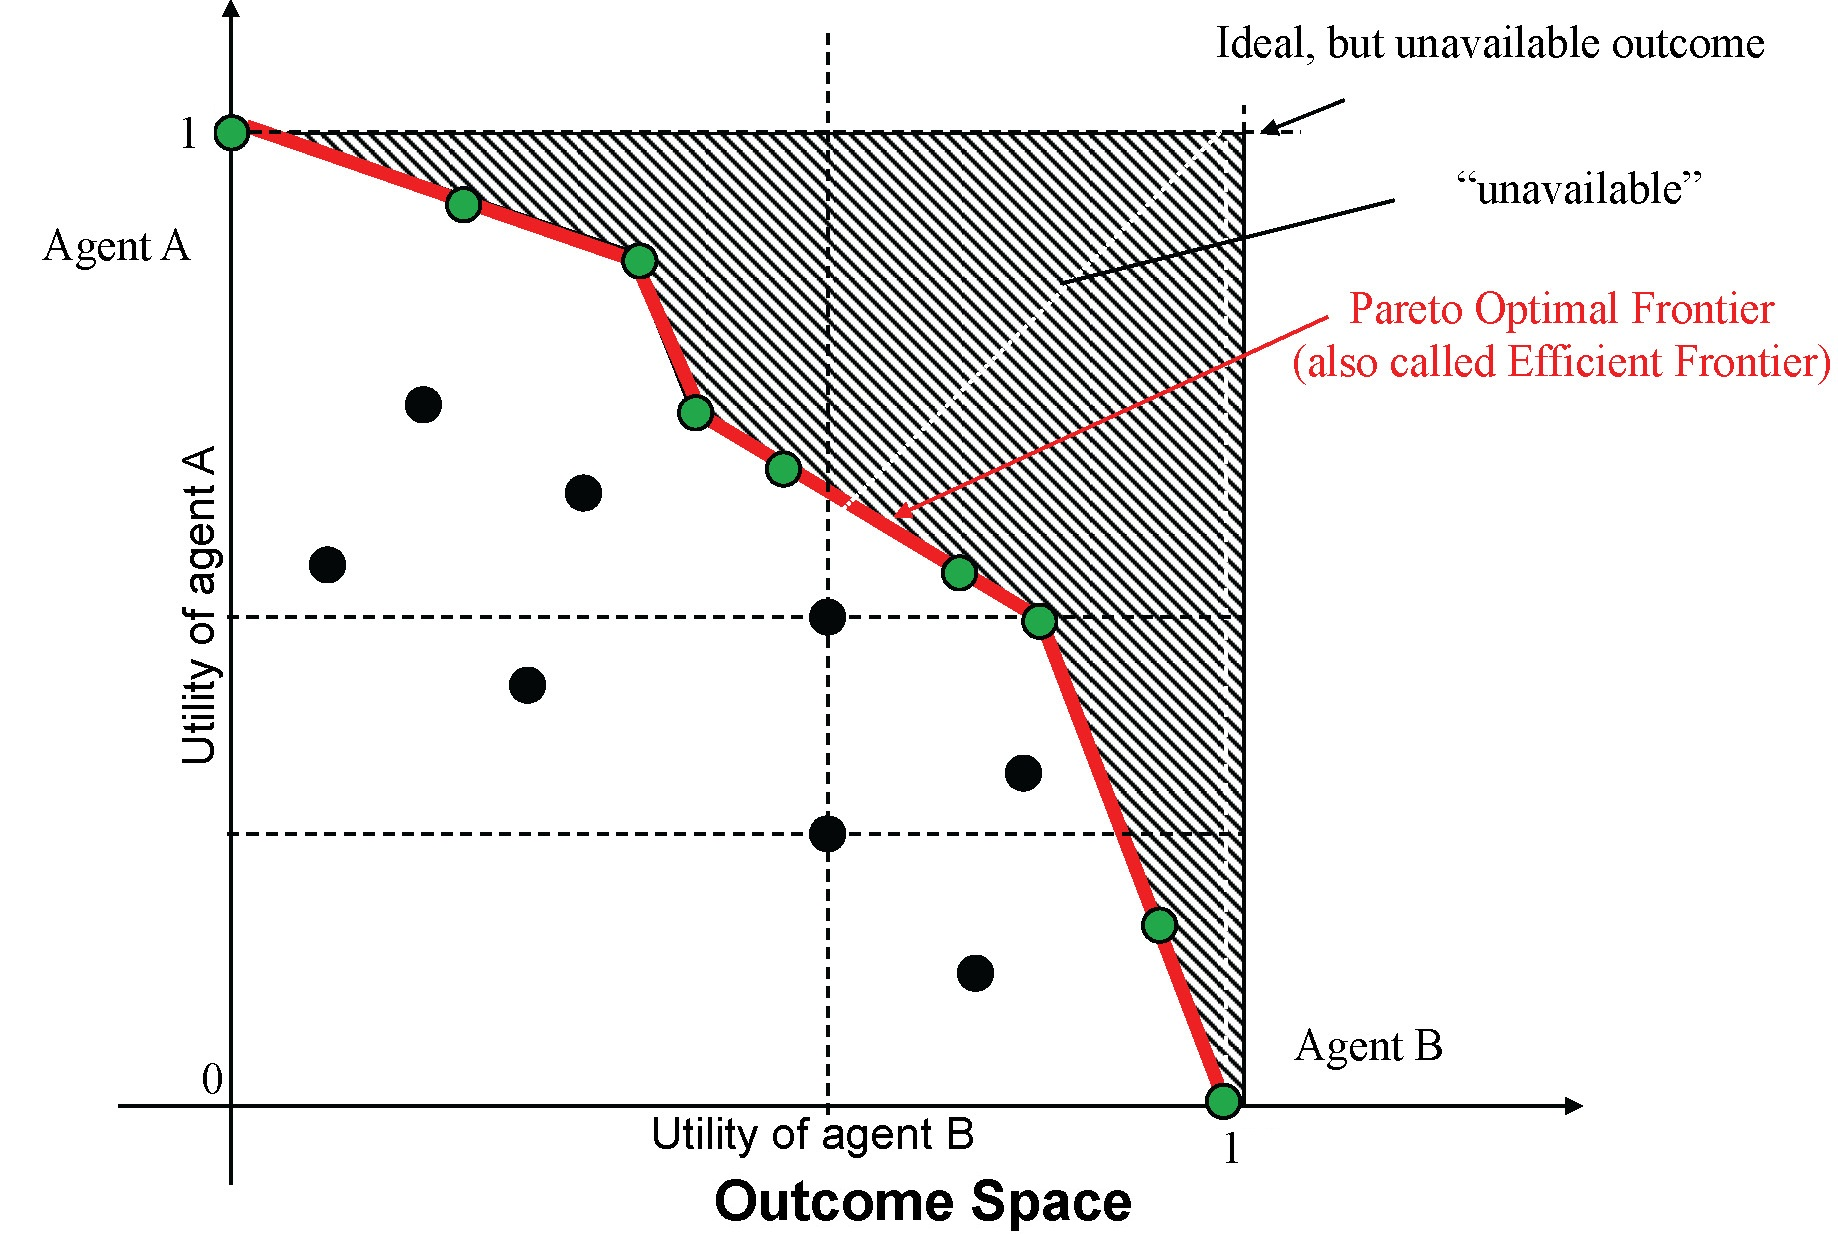
\includegraphics[width=10cm]{OutcomeSpace.pdf}

\includegraphics[width=10cm]{party.jpg}
\caption{Organizing a party involves choosing music, food, drinks, catering, etc.}\label{fig:party}
\end{figure}

This document describes the practical assignment for the second quarter of the AI course. The practical assignment aims at familiarizing students with parts of the course material in a more practical way. This assignment is about {\em negotiation}. Negotiation is a form of interaction in which two (or more) agents, with conflicting interests and a desire to cooperate, try to reach a mutually acceptable agreement. Negotiation between two agents can in many ways be modeled as a game, and game theory is useful to analyze the behavior of negotiating agents. Negotiation is, however, also different from many board games such as chess and reversi. One of the most important differences is that negotiation as we will study it in this practical assignment never is a zero-sum game. That is, a typical negotiation does not have a winner who takes all and a loser who gets nothing. In order to start a negotiation, it is only reasonable for both parties to believe that there is a {\em win-win} situation where both agents can gain by obtaining a deal through negotiation. Another difference is that the domain of negotiation (what the negotiation is about) may be quite different from one negotiation to the other.

To clarify, we add some remarks about the {\em process} of negotiation. Typically, negotiation is viewed as a process divided into several phases. Initially, in a {\em prenegotiation phase} the negotiation domain and the issue structure related to the domain of negotiation are fixed. Negotiation may be about many things, ranging from quite personal issues such as deciding on a holiday destination to strictly business deals such as trading orange juice in international trade. In this assignment, the party domain has been selected and the structure of this domain is provided to you. In other words, the prenegotiation phase has been completed and you cannot redefine the domain anymore. There are two tasks that are usually considered part of the prenegotiation phase that you do need to consider in this assignment. The first task involves creating a so-called {\em preference profile} that captures your own preferences with regards to the party domain. The result will be a formal preference function that maps each possible {\em outcome} of a negotiation to a {\em utility number} in the range of 0 to 1. The second task involves thinking about a {\em strategy} used to perform the negotiation itself. But the most important part of this assignment concerns the {\em negotiation phase} itself, i.e.\ the exchange of offers between you (or your software agent) and an opponent. Figure \ref{fig:hints} provides some initial guidelines based on human experience with negotiation that may help you during your own negotiations and in building your own negotiating software agent.

\begin{figure}[h]
\begin{center}
\doublespacing
\begin{tabular}{|c|}
\hline
Orient yourself towards a win-win approach.\\
Plan and have a concrete strategy.\\
Know your reservation value, i.e.\ determine which bids you will never accept.\\
Create options for mutual gain.\\
Take the preferences of your opponent into account.\\
Generate a variety of possibilities before deciding what to do.\\
Pay a lot of attention to the flow of negotiation.\\
\hline
\end{tabular}
\end{center}
\caption{Negotiation guidelines}\label{fig:hints}
\singlespacing
\end{figure}

This assignment 
%consists of several parts. First, you will have to think about
%your preferences and each of you will have to {\em individually} define a preference profile for the party domain briefly mentioned above. This profile will be used in grading so it is probably good to advice you to be true to yourself. The domain itself will be provided to you at a later time. Then you will negotiate with another student and a software agent about this domain, with the aim of reaching an agreement while at the same time trying to get an outcome as close to your own preferences as possible. Finally, the largest part of this assignment 
concerns building your own negotiating software agent. This will be a {\em team effort}: as a team you will
design and implement your negotiating agent in Java to do negotiations for you.

Some techniques relevant for building and designing negotiating agents can be found among others in chapters 16 and 17 in \cite{Rus033rd}. The assignment will also require you to go beyond the course material in the book. Additional information is provided to you in the form of several papers \cite{Baarslag12ACAN,Jon01,Lin12,Far98,Ser05}. There is a lot of other literature available about negotiation that may help you finish this assignment successfully. As for almost any subject, you can find more information about negotiation strategies online. We recommend to search for strategies used in the ANAC competition~\cite{ANAC2011Baa,ANAC2011Ada,ANAC2011Dir,ANAC2011Fis,ANAC2011Frie,ANAC2011Kaw,ANAC2011Kri,ANAC2011Wil}.

The remainder of this document is organized as follows. In Section~\ref{sec:assignment} the objectives, deliverables, requirements and assignment itself are described. Section~\ref{sec:organization} describes some organizational details and important dates, including deadlines. Finally, Section~\ref{sec:evaluation} documents the evaluation criteria and grading for this assignment.

\section{Detailed Assignment Description}\label{sec:assignment}
The assignment must be completed in teams of 4 or 5 students. In the following paragraphs the objectives, deliverables, requirements, and the detailed assignment description are documented.

\subsection{Objectives}
\begin{itemize}
\item To learn to design a negotiating agent for a realistic domain with both discrete and integer issues, including among others a negotiation strategy.
\item To learn techniques for implementing (adversarial) search and design heuristics while taking into account time constraints.
\item To actively interact with other students and participate in student groups by discussing and coordinating the design and construction of a negotiating agent.
\end{itemize}


\subsection{Deliverables}

\begin{itemize}
\item A unique number $n$ to identify the team and the negotiating agent (which will be provided to you after registering your group). You may opt to use the same team as the first assignment.
\item A negotiating agent programmed in Java using the negotiation environment provided to you consisting of the following components:
  \begin{itemize}
    \item A package containing your agent code: both the class and src files. It is obligatory to use the package ``negotiator.group''~+~$n$ for the negotiating agent and any other required files. An agent consists of four components and optionally several helper classes. For example for group 3 the package should at least include: \textit{Group3\_BS} (bidding strategy), \textit{Group3\_AS} (acceptance strategy),\textit{ Group3\_OM} (opponent model), and \textit{Group3\_OMS} (opponent model strategy).

 In addition, a custom \textit{BOArepository.xml} should be included specifying the components with optionally their parameters.
  \end{itemize}
\item A report documenting and explaining the solution.
%\item A PPT presentation, to be presented at the end of this assignment, taking no longer than 4 minutes.
\end{itemize}

The report need not be lengthy (10 A4 pages may be enough, 15 A4 pages maximum), but should include an explanation and motivation of {\em all} of the choices made in the design of negotiating agent. The report should also help the reader to understand the organization of the source code (important details should be commented on in the source code itself). This means that the main Java methods used by your agent should be explained in the report itself.

     Please make sure all your files are in the directory structure as explained above. Assuming that the group has number three, a valid directory structure is:

\begin{enumerate}
	\item[] boarepository.xml\vspace{-0.3cm}
	\item[] Group3\_report.pdf\vspace{-0.3cm}
	\item[] negotiator/\vspace{-0.3cm}
	\begin{enumerate}
		\item[] group3/\vspace{-0.1cm}
		\begin{enumerate}
			\item[] Group3\_AS.class\vspace{-0.1cm}
			\item[] Group3\_AS.java\vspace{-0.1cm}
			\item[] Group3\_BS.class\vspace{-0.1cm}
			\item[] Group3\_BS.java\vspace{-0.1cm}
			\item[] Group3\_OM.class\vspace{-0.1cm}
			\item[] Group3\_OM.java\vspace{-0.1cm}
			\item[] Group3\_OMS.class\vspace{-0.1cm}
			\item[] Group3\_OMS.java\vspace{-0.1cm}
			\item[] SomeHelperClass.class\vspace{-0.1cm}
			\item[] SomeHelperClass.java\vspace{-0.1cm}

		\end{enumerate}
	\end{enumerate}
\end{enumerate}



\subsection{Requirements}
\begin{itemize}
\item The agent should implement a negotiation strategy to generate offers, and an acceptance strategy to decide whether to accept an offer or not.
\item The agent must aim at the best negotiation outcome possible (i.e. the highest score for itself given the agent's preferences, while taking into account that it may need to concede to its opponent).
\item The agent must take the utility of the opponent into account. Of course, initially you only have information about your own preferences. You will have to \emph{learn} the preferences of the opponent during the negotiation process. The default way is by constructing an \emph{opponent model} to have an idea of the utility of your proposed bids for the opponent. We already provided an opponent model, which you are asked to improve.
\item The agent meets reasonable time and memory constraints. Any agent that uses more than a minute in order to initiate the negotiation or to reply to an opponent's offer will be disqualified.
\item Make sure your agent is able to work on at least all given scenarios. You may assume that the domains solely contain \emph{discrete} or \emph{integer} issues. You may also find references in the negotiation environment to \emph{reservation values}, but you can ignore these, as they do not play play a role in this assignment.
\item The source code should contain explanatory comments that will allow third parties not involved in programming the code to understand it. A clear explanation of a method must be provided at the beginning of every method. Parts of the code that are not self-explaining should receive additional documentation. Please incorporate enough information in comments in the code to ensure this. Finally, make sure that you have removed all debug printouts from your code and that your agent does not flood the 'System.out' channel.
\item The agent implementation should be tested to ensure that it works on multiple systems, and requires nothing other than the files contained in your group's package. Integrating your agent into the negotiation environment should not be more difficult than adding your package (e.g. the folder ``negotiation/group$n$/'') in the right folder (the same directory in which the negotiation simulator \verb|negosimulator.jar| can be found).
\item The report should include:
  \begin{itemize}
    \item the group number,
    \item an introduction to the assignment,
    \item a high-level description of the agent and its structure, including the main Java methods (mention these explicitly!) used in the negotiating agent that have been implemented in the source code,
    \item an explanation of the negotiation strategy, decision function for accepting offers, any important preparatory steps, and heuristics that the agent uses to decide what to do next, including the factors that have been selected and their combination into these functions,
    \item a section documenting the tests you performed to improve the negotiation strength of your agent. You must include scores of various tests over multiple sessions that you performed while testing your agent. Describe how you set up the testing situation and how you used the results to modify your agent,
    \item answers to the questions posed in the assignment, and
    \item a conclusion in which you summarize your experience as a team with regards to building the negotiating agent and discuss what extensions are required to use your agent in real-life negotiations to support (or even take over) negotations performed by humans.
  \end{itemize}
\end{itemize}

\subsection{What is provided to you as a start?}\label{sec:implementation}

The following items are provided to you to help you complete the assignment.
\begin{itemize}
  \item This document, called \verb|assignment.pdf|,
  \item A user guide, called \verb|userguide.pdf| for the negotiation environment,
  \item A negotiation environment called Genius including example agents and scenarios,
  \item The source code of the agent \verb+SimpleAgent+,
  \item The source code of four BOA components: bidding strategy \verb+TimeDependent_Offering+, acceptance strategy \verb+AC_Next+, opponent model \verb+HardHeadedFrequencyModel+, and opponent model strategy \verb+BestBid+.
\end{itemize}

\subsection{Assignment}
In this section, the main tasks and questions you need complete are presented. But before we do this, we present additional background that may help you to complete this assignment successfully. Please start by making yourself familiar with the negotiation environment \cite{Lin12} (start and use \textit{negosimulator.jar})  and read the user guide (\textit{userguide.pdf}) as well as this assignment provided to you carefully. Note that the negotiation environment is a scientific software tool which is being improved constantly. Please report any major bugs found so that we can resolve them in a next version.
%Genius can be downloaded from:
%\begin{center} 
%\verb+http://mmi.tudelft.nl/negotiation/index.php/Genius+
%\end{center}


A negotiation in this assignment is also called a {\em negotiation session}. In a session two agents negotiate with each other to settle a conflict and negotiate a deal. Each negotiation session is limited by a fixed amount of time. At the end of a session, a score is determined for both agents based on the utility of the deal for each agent if there is a deal, otherwise the score equals the reservation value; in this assignment 0.0. In a sense, there is no winner since each agent will obtain a score based on the outcome and its own utility function. A failed negotiation, in the sense that no deal is reached, thus is a missed opportunity for both agents. In the tournament that will be played, each agent will negotiate with all other agents and the scores of each session are recorded and averaged to obtain an overall score for the agent (see Section \ref{sec:evaluation}). A ranking will be compiled using these overall scores.

%The main reason for multiple negotiation sessions is that agents may learn about their opponent from the sequence of bids exchanged and from the negotiation outcome (e.g. deal or no deal). Exchanging offers allows the parties to learn about the others' limitations, and to identify the key issues and critical areas of disagreement. During this phase, the parties realize the potential of a compromise and can assess its main features. The analysis of a negotiation may focus on the modification of strategies, the determination of concessions, and on the restriction of efficient solutions to those which may be acceptable to the parties. A second reason for having multiple sessions (where in the tournament only the last session will be scored) is that it will sometimes be useful to break off the negotiation to signal dissatisfaction about the way negotiation proceeds to the other agent.

Key to this assignment is the fact that you have incomplete information about your opponent. You may assume that there is a conflict of interests, but at the start you do not know on which issues agents agree and on which they disagree. For example, in a negotiation about buying a laptop the buyer may prefer to have a middle-sized screen but the seller may prefer to sell laptops with small screens because (s)he has more of those in stock. They could, however, agree on the brand of laptop that they want to buy/sell. An outcome of a negotiation reconciles such differences and results in an agreed solution to resolve the conflict.

Ideally, such an outcome has certain properties. One of these properties is that the outcome should be Pareto optimal. An outcome is Pareto optimal when there does not exist a deal where one agent can do better and one can do better or the same (i.e.\ they both score higher or equal, and therefore both would prefer this new deal over the old one). Another property is related to the Nash solution concept. A Nash solution is an outcome that satisfies certain bargaining axioms and may be viewed as a ``fair outcome'' which is reasonable to accept for both parties. An outcome is said to be a Nash solution whenever the product of the utility (in the range $[0, 1]$) of the outcome for the first agent and that for the second agent is maximal (cf. \cite{Ser05}). The notion of a fair outcome is important in negotiation because it provides a reference point for what your opponent might be willing to accept. Typically, a negotiation is started since reaching an agreement is better than not. But in order to get an agreement, you will need to get your opponent to agree. In a negotiation between self-interested agents, however, each agent is determined to get the best possible outcome for itself.

The Nash solution concept, as it is called, excludes certain outcomes as being unfair. It is, for example, very unlikely that your opponent will accept an offer that is most favorable to you and leaves your opponent with empty hands. In general, it is to be expected that an outcome is the result of a number of concessions that both parties make. Concessions can be made in various ways, quite easily or more slowly. The speed of making concessions, or the concession rate is the derivative of the (size of the) concession steps taken during a negotiation. An agent that makes concessions in very small steps initially uses a so-called Boulware strategy. A strategy that makes faster concessions  initially is called a Conceder. Other strategies are conceivable and may be necessary given the deadlines (cf. \cite{Fat01}).

To compute whether a bid in a negotiation is Pareto optimal or a Nash solution we use so-called {\em utility functions} (cf. \cite{Rus033rd}). In our case, utility functions assign quantitative values to bids in the negotiation space. In this assignment, you may assume that all utility functions are additive, i.e.\ they will always be linear in the number of issues. For example, if there are four issues to negotiate about, the utility function can be computed by a {\em weighted sum} of the values associated with each of these issues. So, let $bid=\langle i_1,i_2,i_3,i_4\rangle$ be a particular bid. Then the utility $u(bid)=u(i_1,i_2,i_3,i_4)$ (given weights $w_1,w_2,w_3,w_4$) can be calculated by: 
\[
    u(i_1,i_2,i_3,i_4) = w_1\cdot u(i_1)+w_2\cdot u(i_2)+w_3\cdot u(i_3)+w_4\cdot u(i_4)
\]

The outcome space of a negotiation, i.e.\ all possible bids, can be plotted on a graph which indicates the utility of both agents on the $x$ and $y$ axes respectively. An example is provided in Figure \ref{fig:OutcomeSpace}.

%\begin{center}
\begin{figure}[h]
\centering
%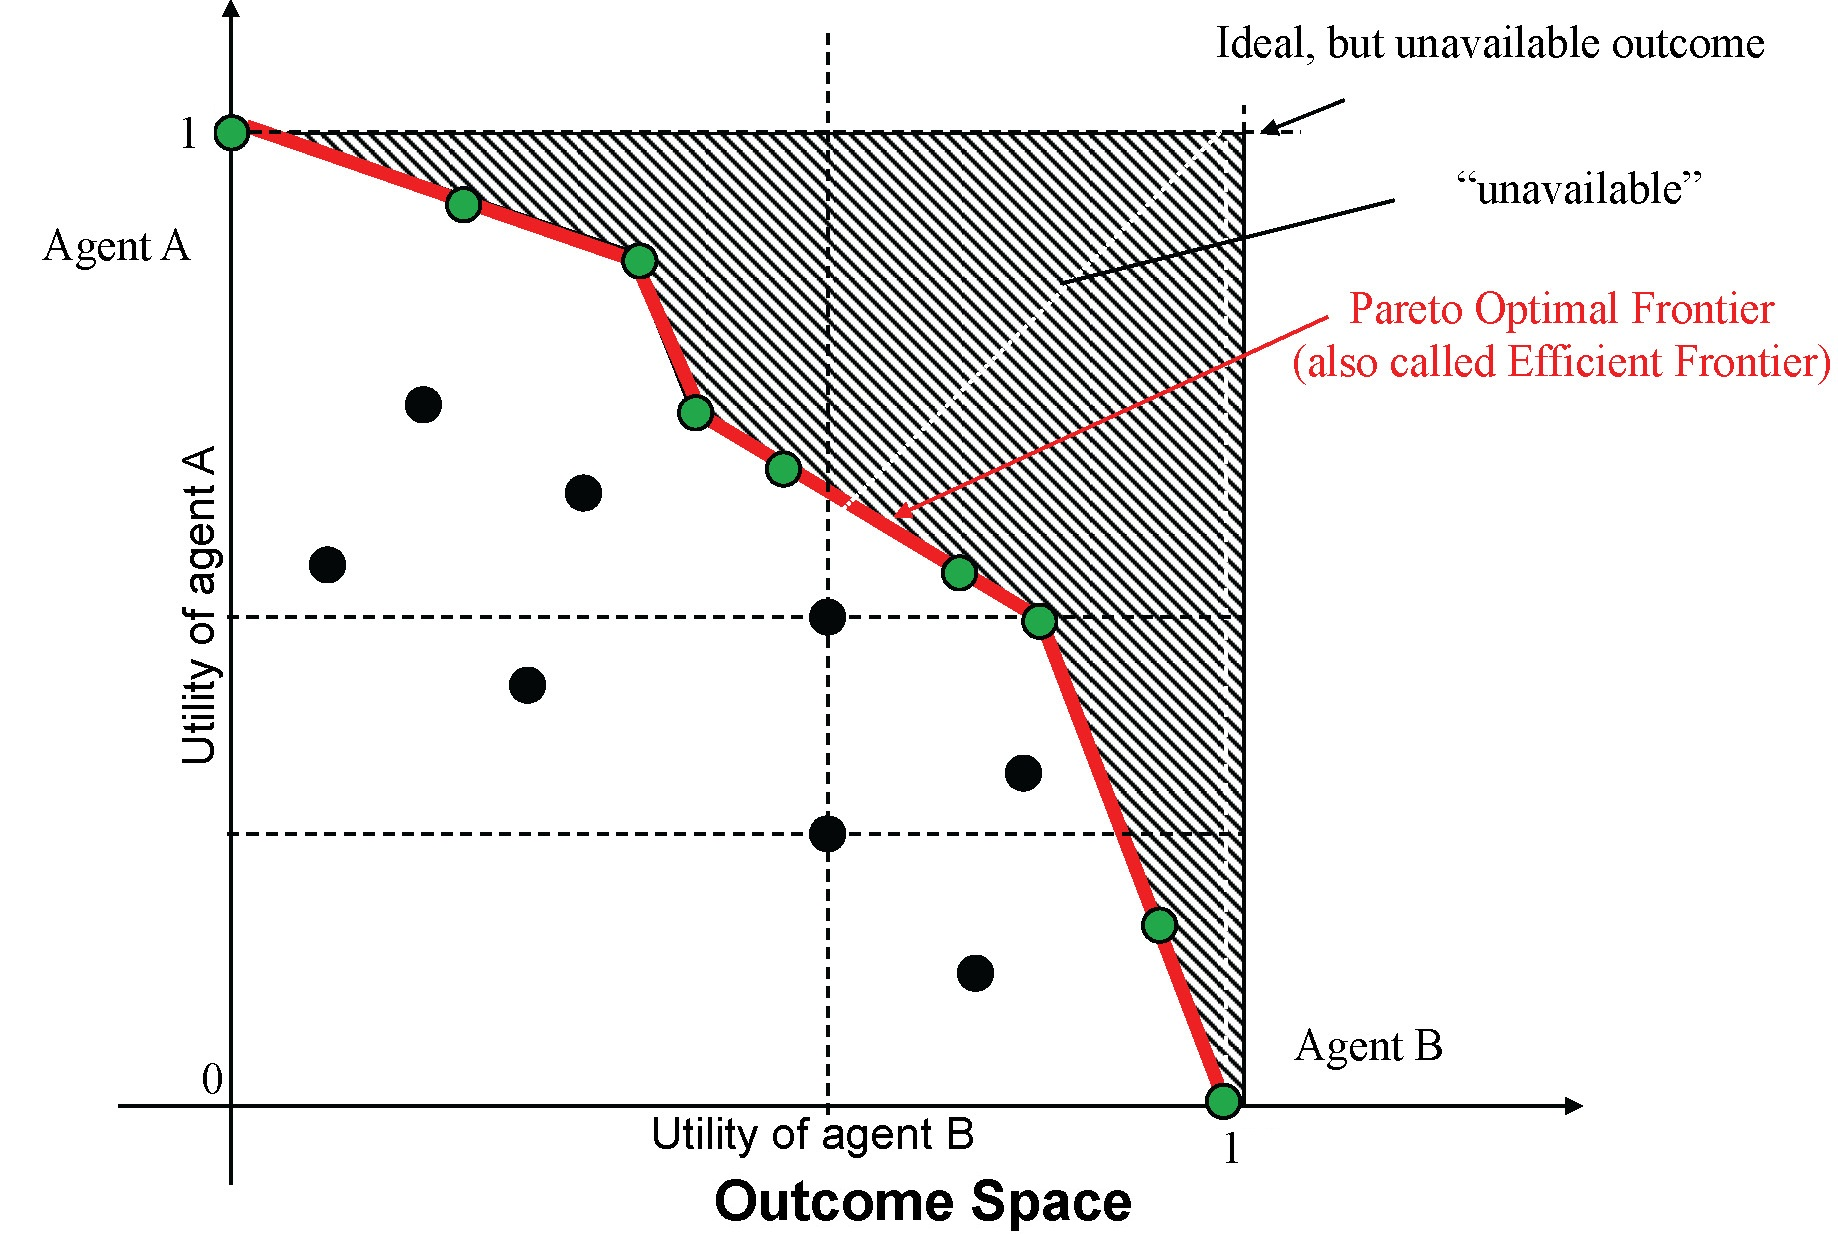
\includegraphics[width=10cm]{OutcomeSpace.pdf}
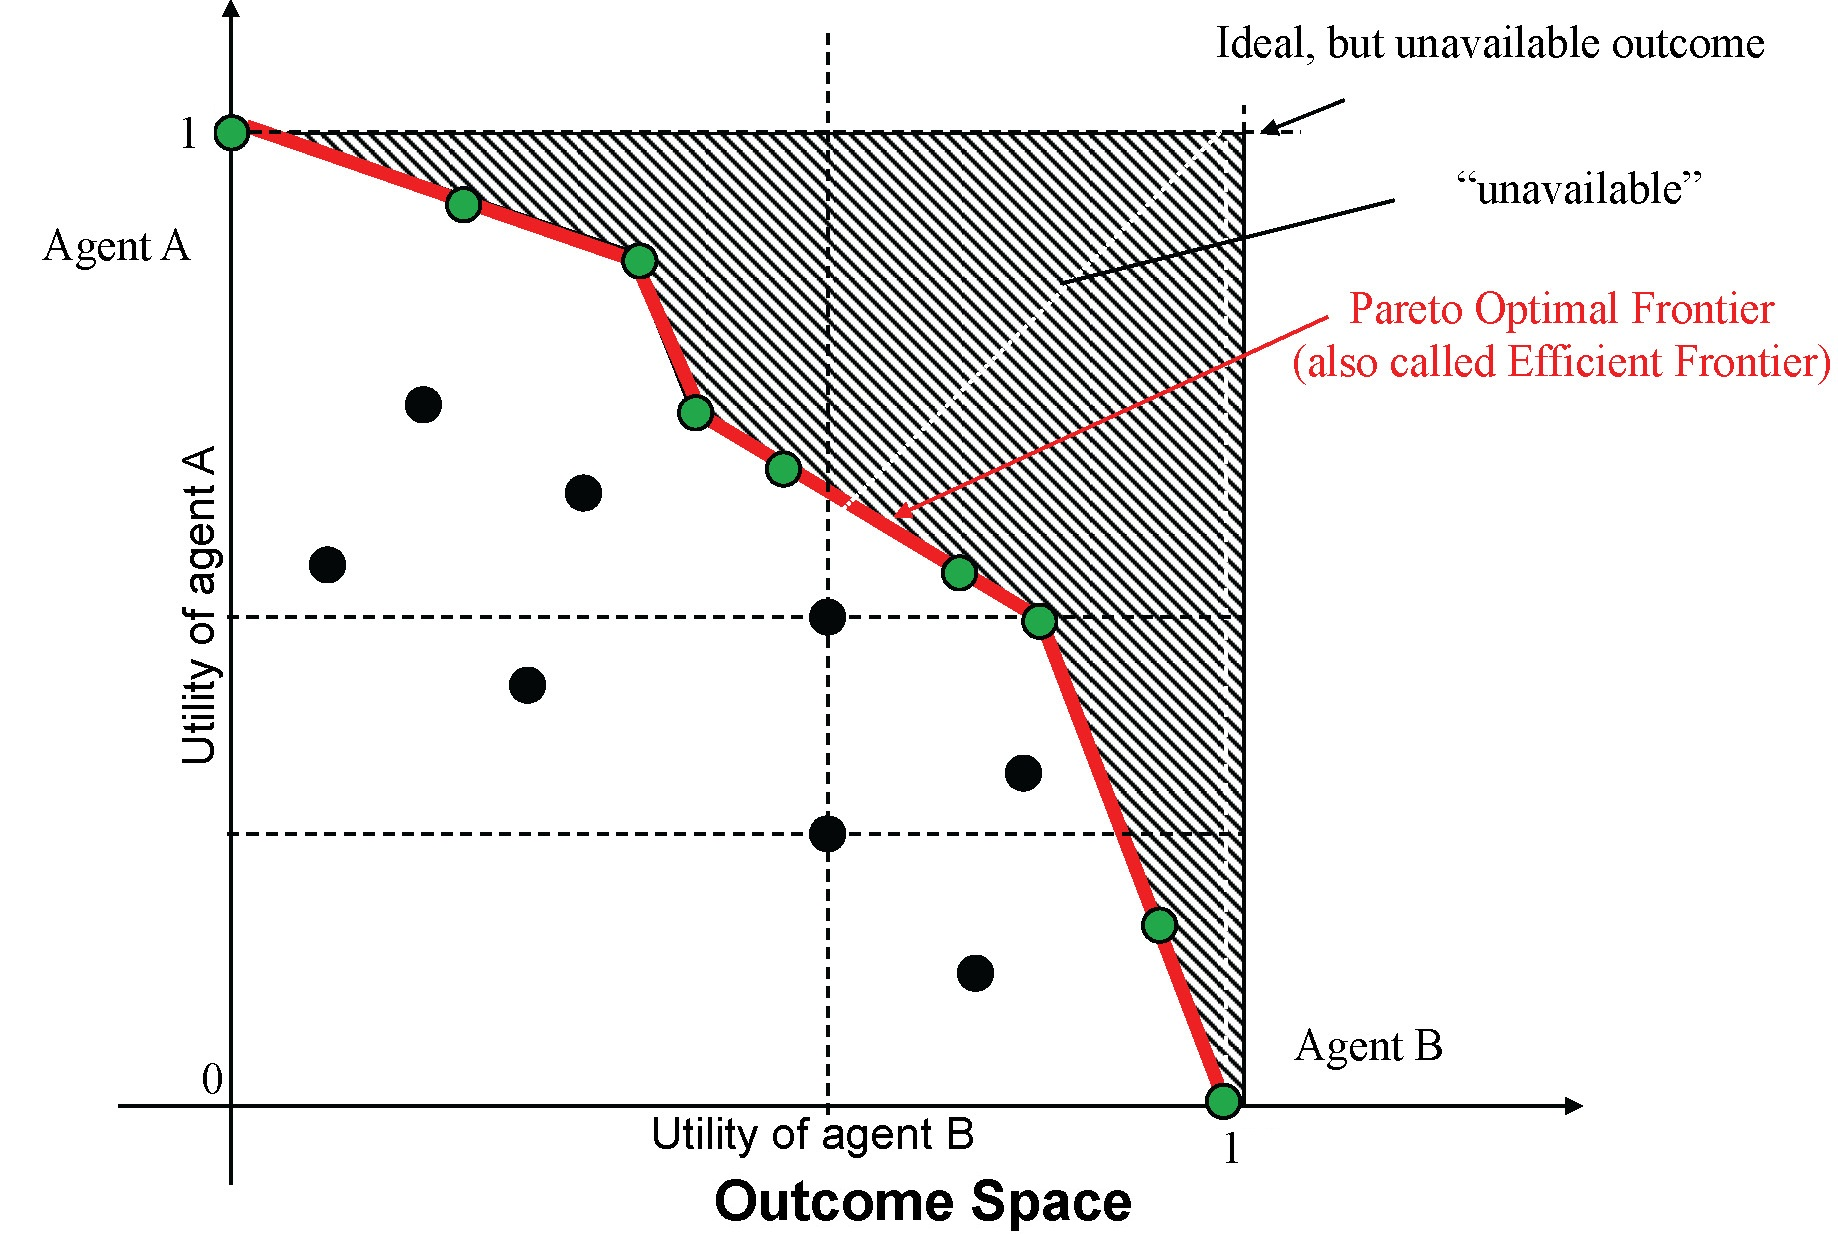
\includegraphics[width=10cm]{OutcomeSpace.jpg}
\caption{Pareto Frontier}\label{fig:OutcomeSpace}
\end{figure}
%\end{center}

What sets the negotiations considered in this assignment apart from other negotiations is the fact that both agents have exactly the same deadline for achieving a deal and both agents ``know'' this.

Finally, the negotiation domain may also contain \emph{discount factors}. Discount factors model the fact that the desirability of the good being traded may decline with time. This happens when the good is perishable, for example due to inflation. The implementation of discount factors is as follows. Let $d$ in $(0, 1]$ be the discount factor of a domain, and $\omega$ be a certain outcome. Let $t$ in $[0, 1]$ be the current normalized time, as defined by the timeline. We compute the discounted utility $U_{discounted}^t$ as follows:

\begin{eqnarray}
U_{discounted}^t(\omega) = U_{undiscounted}(\omega) \cdot d^t
\end{eqnarray}
%At $t = 1$, the original utility is multiplied by the discount factor.  Furthermore, 
The presence of a discount factor means that the value of reaching an agreement is time-dependent. Hence, the agents should try to reach an agreement sooner rather than later. To be clear, the discount factors depend on the domain, but the deadline is fixed and is set to three minutes, and both agents share this fixed time window. 

If $d = 1$ or not present at all (in which case $d=0$), the utility is not affected by time, and such a domain is considered to be undiscounted, while if $d$ is very small there is high pressure on the agents to reach an agreement immediately. Note that in our set-up, discount factors are part of the preference profiles and therefore in general differ between agents.

The assignment consists of first familiarizing yourself with the negotiation environment and then designing and implementing a negotiating software agent. You do not have to discuss the questions \emph{(i)} - \emph{(vii)} in your report.

\subsubsection{Familiarizing Yourself With the Negotiation Environment}

\begin{enumerate}
    \item[i.] Read the userguide for the negotiation environment. In order to familiarize yourself with the environment, complete the items below.
	\item[ii.] Inspect the negotiation templates named \verb|laptop_domain.xml|, \verb|laptop_buyer_utility.xml| and \verb|laptop_seller_utility.xml| in the GUI. Make a new preference profile for buying a laptop and edit the preferences according to your own preferences.
    %compute the utilities for all the possible bids in the outcome space and plot them on a graph such as Figure \ref{fig:OutcomeSpace}    
	\item[iii.] Create a new negotiation session. For the agents choose the \verb|SimpleAgent| and the \verb|UIagent|. Select two different preference profiles of the Laptop domain and start the negotiation. Familiarize yourself with running a negotiation and note the difference between both agents: the \verb|SimpleAgent| is automated, whereas  \verb|UIagent| asks the user for input. You may want to repeat this exercise using two automated agents.
	\item[iv.] Analyze the performance of the \verb|SimpleAgent| in the laptop domain by letting it play against itself. Is a Pareto optimal outcome reached? Think about why it obtains the outcome that it does.

	\item[v.] Now we know how to run a single negotiation session, it is time to run a tournament. In the user guide it is discussed how to run a tournament. Specify a simple tournament with the following parameters:
	\begin{itemize}
		\item \textbf{Protocol}: ``Alternating offers''.
		\item \textbf{Preference profiles}: both preference profiles of ``Amsterdam''.
		\item \textbf{Agent side A}: ANAC2011 - HardHeaded.
		\item \textbf{Agent side B}: Other - TDT Conceder.
		\item \textbf{Number of sessions}: 1.
		\item \textbf{Tournament options}: \textsc{Protocol mode}: \textit{time}; \textsc{Deadline (seconds)}: \textit{60}; \textsc{Access partner preferences}: \textit{false}; \textsc{Allow pausing timeline}: \textit{false}; \textsc{Play both sides}: \textit{true}; \textsc{Play against self}: \textit{false}; \textsc{Log detailed analysis}: \textit{true}; \textsc{Log negotiation trace}: \textit{false}; \textsc{Log final accuracy}: \textit{false}; \textsc{Log competitiveness}: \textit{false}, \textsc{Append mode and deadline}: false; \textsc{Show all bids}: \textit{true}; \textsc{Show last bid}: \textit{true}; \textsc{Disable GUI}: \textit{false}.
		\item \textbf{BOA Agent side A/B}: null.
	\end{itemize}
	After running your tournament there should be two logs in the log directory. As the logs are in XML format, you can easily analyze them by importing them in Excel and using pivot tables. Note that these features are only available in the full version of Excel (no starter). This version can be found on for example the TU Delft computers. 
	\item[vi.] Using a similar method as above, we can also run a tournament featuring BOA agents. The difference between a normal agent and a BOA agent is that a BOA agent consists of four components: a bidding strategy, an acceptance strategy, an opponent model and an opponent model strategy. A large set of components is included in Genius and we can simply create a BOA agent by selecting a component of each type.

Use the same configuration but remove all agents from agent side A. Next, add a single BOA agent with the following components: Bidding strategy: \textit{2011 - Agent K2}; Acceptance strategy: \textit{Other - next}; Opponent model: \textit{HardHeaded Frequency Model}; Opponent model strategy: \textit{Best bid}. Run the tournament and analyze the results. Note that if we specify both normal agents and BOA agents on side A, then the sets are merged and treated as a single set of agents.
	\item[vii.] Finally, check the JavaDoc of the classes discussed in the userguide in Section ``Overview of Classes''.
\end{enumerate}

\subsubsection{Design and Implement a Negotiating Software Agent}

The remainder of this assignment concerns the design and implementation of a negotiation agent. This negotiating agent will be tested on a large set of scenarios, of which some are made available to you.

\begin{enumerate} 
%\setcounter{enumi}{5}
\item \textsc{Preparation: Analyze Party Domain}

  \begin{enumerate}
  \item Using the GUI, inspect the negotiation template named \verb|party_domain.xml| and the utility profiles that are provided to you in the negotiation environment bundle. 
  %on Blackboard (on \preferenceprofilesonlinedate). 
  Compute and draw the efficient frontier in a graph such as Figure \ref{fig:OutcomeSpace} for two of the templates provided to you.
    \item Analyze the performance of the agent \verb|SimpleAgent| in the party domain playing against itself. Is a Pareto optimal outcome reached? Explain your answer. Also explain why it obtains the resulting outcome that it does. Do the same for the agents \verb|Boulware| and \verb|Conceder|.
  \end{enumerate}
  \item \textsc{Design and implement a negotiation strategy}\\ \break
In this section you have to design and implement your negotiation agent using the BOA framework. Before doing so, it is recommended to read about existing strategies for a similar environment (cf. \cite{ANAC2011Baa,ANAC2011Ada,ANAC2011Dir,ANAC2011Fis,ANAC2011Frie,ANAC2011Kaw,ANAC2011Kri,ANAC2011Wil}).
  \begin{enumerate}
    %\item Decide on the way your agent will set a {\em reservation value}. Explain in the report informally how your agent determines its reservation value and describe how you implemented this in your agent. In case your agent also uses other considerations to determine whether it will never accept particular bids, also explain these considerations.
 	 \item Create a PEAS description in the same format of a table as in \cite{Rus033rd} of the negotiating agent that you need to design and implement in this assignment. Use this negotiation assignment setup as the task environment. Be as complete as possible and pay special attention to the performance measure of the agent. Also include a brief discussion about each element included in your PEAS description. In particular, explain informally what goals the agent has in a negotiation.

 	 \item For implementing the agent we will be using the BOA agent framework as discussed in~\cite{Baarslag12ACAN} and the userguide. The main advantage of this framework is that you can benefit from using a large set of existing components. Provide a small description of the role of each component in the BOA framework.
        \item Implement the \textbf{bidding strategy} (Group\textit{n}\_BS). Decide on the way your agent will make its first offer and counter offers. Explain why you have chosen this to be the agent's opening bid and how your agent computes a counter offer. List all considerations that your agent takes into account explicitly and explain why you have chosen to base the agent's decision on these considerations.

Does your agent ever propose offers that {\em increase} the utility for itself relative to its previous bid? If not, demonstrate that the utility associated with bids in any bid sequence your agent will ever propose in a negotiation monotonically decreases. If it does, explain when and why it will decide to do this.

Finally, the source and compiled class should be placed in the folder ``negotiator/group3/'' relative to the root of Genius as ``Group3\_AS.class'' and ``Group3\_AS.java'' and added to the BOA repository.

        \item Implement the \textbf{acceptance strategy} (Group\textit{n}\_AS). Describe which factors the agent takes into account for making this decision. Does your agent take time and/or opponent's actions into account when deciding to accept an offer? In case your agent also uses other considerations to determine whether it will accept particular bids, also explain these considerations.
       \item Implement the \textbf{opponent model} (Group\textit{n}\_OM). For this assignment we included the source code of the \textit{HardHeaded Frequency Model}. Frequency models learn the issue and value weights of the opponents preference profile separately. The issue weights are calculated based on the frequency that an issue changes between two offers. The value weights are calculated based on the frequency of appearance in offers.

While the model is among the best known opponent models, it could be better. Initially, the quality of the opponent model is increases over time. However, after a small amount of time passed, the model actually becomes less accurate over time. Describe how you would improve the given model and implement your changes. Explain why you believe your changes result in a better model.

	\item Implement the \textbf{opponent model strategy} (Group\textit{n}\_OMS). For this assignment you may improve the opponent model strategy ``Best bid'' which is included in this distribution or design your own opponent model strategy. A hint for an alternative implementation is to keep in mind that opponent models are imperfect.
  \end{enumerate}

  \item \textsc{Quantify the performance of your agent}
      \begin{enumerate}
        \item Have your agent negotiate against itself, and against the three ANAC2011 agents \textit{HardHeaded}, \textit{Gahboninho}, and \textit{TheNegotiator} provided to you on the party domain. Run several negotiation sessions using various utility profiles. Report on the outcomes reached. Try to explain why the outcome is as it is. Are any of the outcomes a Nash solution? Is it possible to reach an efficient outcome, i.e.\ an outcome that lies on the Pareto Frontier?
	\item Test your agent in a small tournament while varying the acceptance strategy. Is there an acceptance strategy which is better than your acceptance strategy?
	\item Test your agent in a small tournament and compare your opponent model with the original HardHeaded frequency model. Does your model lead to a significantly higher utility?
        \item One important question remains. How generic is your agent? That is, does it work as well on the party domain as on other domains? To verify this, have your agent negotiate against itself, and against at least three agents provided to you on at least three scenarios (for example, {\em Laptop}, \emph{Grocery} and {\em ADG}). Make sure your agent is able to deal with discounted domains. Report on the outcomes reached. Try to explain why the outcome is as it is. Is any of the outcomes a Nash solution? Is it possible to reach an efficient outcome, i.e.\ an outcome that lies on the Pareto Frontier?
      \end{enumerate}
\end{enumerate}


\subsubsection{Concluding: Future Perspectives}

\begin{enumerate}
\setcounter{enumi}{3}
  \item As you will have noticed by now, it is hard to find deals that are Pareto optimal. An alternative for one-to-one negotiation as used in this practical assignment is to use a trusted mediator to which each agent declares its private preferences. The mediator then will compute an efficient outcome using this input. Do you think that introducing a mediator is a better option for finding an optimal outcome for both agents? If so, argue why you think so and describe the circumstances in which it is particularly suitable to use a mediator. If not, argue why you think it is not useful to do this.
  \item The agents in the negotiation environment have limited capabilities in order to achieve a negotiated deal. Think about capabilities (e.g.\ other actions or forms of communication) that an agent might be extended with. Can you think of additional capabilities that would help an agent to achieve a better deal? If so, explain why these capabilities would help an agent to achieve a better deal. If not, argue why there will not be any capabilities that could help an agent achieve a better deal.
\end{enumerate}

As a final remark, we want to make clear that it is very important to test your agent in order to improve the negotiation strength of your agent. A warning is in place though: do not assume that your goal is to outperform a `stupid' agent'. Try to beat all ANAC2011 agents and older versions of your own agent. A good outcome is determined by other criteria, identified by efficiency of the outcome (i.e.\ is it close or not to the Pareto Frontier). To test your agent in this regard, it will in particular be useful to test your agent on various negotiation templates. You can create these templates both by modeling real-life examples of negotiation or create them randomly. 

In general, there are many techniques to improve the negotiation strength of agents. Various factors can be taken into account when deciding on acceptance, breaking off, or computing a next offer in a negotiation, for example you can take into account the time an opponent takes to reply with a counter offer, the consistency of an opponent's offers, the concession rate of your opponent, the history of previous negotiation sessions, and possibly other considerations about the domain of negotiation itself. If your agent performs well enough, you could even participate in the yearly competition for automated negotiating agents, called ANAC~\cite{Baarslag10ANAC}\footnote{\url{http://ii.tudelft.nl/anac}}. A student team of this course won the competition in 2011 and won \$1000,-.
 
\section{Organization}\label{sec:organization} 

You may only use the e-mail address below to submit deliverables to the assignment or ask questions.
\paragraph{Important Dates:}
\begin{enumerate}
  \item {\bf \groupdate}: Deadline for registering your group. Please send an e-mail to 
  \begin{center}
  \verb+ai@ii.tudelft.nl+
  \end{center}
  listing your group members, and we will assign a group number to you.

\item {\bf \deadline}: Deadline for submitting your team solution including a negotiating software agent and report.\\\break
  Please submit your report in PDF format and the package for your negotiating agent by mail to \texttt{ai@ii.tudelft.nl}. Use the naming conventions described elsewhere in this document, including your group number. Do not submit incomplete assignment solutions; only a complete assignment solution containing all deliverables will be accepted. The deadline for submitting the assignment is strict.
%\item {\bf December 20th, 10:45-12:45}: Deliver a presentation about your solution.
\end{enumerate}



\section{Evaluation}\label{sec:evaluation}

Assignments are evaluated based on several criteria. All assignments need to be complete and satisfy the requirements stated in the detailed assignment description section above. {\em Incomplete assignments are not evaluated}. That is, if any of the deliverables is incomplete or missing (or fails to run), then the assignment is not evaluated.

The assignment will be evaluated using the following evaluation criteria:
\begin{itemize}
\item {\em Quality of the deliverables}: Overall explanation and motivation of the design of your negotiating agent; Quality and completeness of answers and explanations provided to the questions posed in the assignment; Explanatory comments in source code, quality of documentation,
\item {\em Performance:} Agents will be ranked according to negotiating strength that is measured in a tournament (see also the next section below),
\item {\em Originality:} Any original features of the agent or solutions to questions posed are evaluated positively. Note that you are required to submit \emph{original} source code designed and written by your own team. Source code that is very similar to that of known agents or other students will not be evaluated and be judged as insufficient. Detection of fraud will be reported to the administration.
\end{itemize}
 

\subsection{Competition}

Agents of teams will be ranked according to negotiation strength. The ranking will be decided by playing a tournament in which every agent plays negotiation sessions against a set of agents -- including the agents programmed by your peers -- on a set of domains. Therefore, your agent should be generic enough to play on any domain. 
%Note that the preference profiles that are collected during the \expdate{} experiment can be used and assigned to agents randomly. 

Agents may be disqualified if they violate the spirit of fair play. In particular, the following behaviors are strictly prohibited: designing an agent in such a way that it benefits some specific other agent, starting new Threads, or hacking the API in any way. 
\subsection{Grading} \label{sec:grading}

Final grades will be determined as a weighted average of several components. The final grade will be determined by your team solution (i.e.\ your assignment, the performance of your negotiating agent and report). 
%, but is also partly based on your individual performance in the negotiation experiment of \expdate. In order to assess individual performance, the preference profile that you create on \expdate{} reflecting your own preferences in the party domain will be used to measure your performance against your fellow students and a negotiating software agent.

The components that are graded and their relative weights are described in Table \ref{tab:grading} below.
\begin{table}[h]
\begin{center}
\begin{tabular}{l p{7cm} c}
\textbf{Assignment} & \textbf{Grading Method} & \textbf{Weight}\\
\hline
\hline
%Human vs.\ Human Negotiation & How well the eventual agreement reflects your profile, i.e.\ how high your utility is with the agreement. If no agreement is reached, the grade will be a 1. & 20\%\\
%\hline
%Human vs.\ Agent Negotiation& Idem, only now you face an electronic negotiation partner. & 20\%\\
%\hline
Negotiating Agent & Performance in a tournament with other agents. & 50\%\\
\hline
Report & Agent design and the final report about your negotiating agent. & 50\%\\
\hline 
\end{tabular}
\caption{\label{tab:grading} Grading criteria and weight}
\end{center}
\end{table}

\subsection{Master Thesis about negotiation}
Did you like thinking about efficient negotiating strategies, or implementing a successful negotiating agent? Negotiation provides a lot of subjects to do your Master Thesis on! You can always ask the course assistants, have a look at the last page of this assignment, or contact us for more information: \verb+negotiation@ii.tudelft.nl+.

\section*{Acknowledgments}
This assignment could not have been written without the help of many people, including T.\ Baarslag, B.\ Grundeken, M.\ Hendrikx, K.\ Hindriks, C.\ Jonker, W.\ Pasman, D.\ Tykhonov, and W.\ Visser.

\bibliographystyle{plain}
\bibliography{references}


\newpage
\begin{center}
\doublespacing
\begin{tabular}{|c|}
\hline
\begin{minipage}{13.5cm}
\hspace{1cm}\\
\textbf{Interested in the possibility of doing a Master Thesis about negotiation?}\\ \\

Negotiation has become a major and interesting research area within Artificial Intelligence. Negotiation is important in many domains ranging from business applications such as Internet market places to incident and crisis management. Negotiation is one of the main tools an autonomous agent has to agree about a course of action or to resolve conflicts with other agents. As such, you might be interested in doing a Master Thesis about negotiation and there are many angles that you can take, e.g.:
\begin{itemize}
\item Design of negotiation strategies and better opponent models (using machine learning techniques);
\item Design of a negotiation support system, either advising humans in a particular domain, or even taking over negotiation all together;
\item Design of a negotiation protocol that can generate better agreements (e.g., multi-agent settings, auctions, use a form of communication between the agents);
\item Design of a testbed for negotiating agents;
\item Extend the current negotiation setting to non-linear utility functions, add dependencies;
\item Design agents in a multi-agent setting, for example an auction;
\item Research related to negotiation, trust and the reputation of agents, either cognitively motivated or viewed from a more engineering point of view;
\item Research on negotiation and culture. How does culture influence negotiation between different agents?
\item Etc.
\end{itemize}
This can all be combined with a Literature Survey course, in order to kick-start your thesis. If you are interested, don't hesitate to ask us: \verb+negotiation@ii.tudelft.nl+ 
\end{minipage}\hspace{.1cm}\\
\hspace{1cm}\\
\hline
\end{tabular}
\end{center}
\singlespacing


\end{document}
